% Options for packages loaded elsewhere
\PassOptionsToPackage{unicode}{hyperref}
\PassOptionsToPackage{hyphens}{url}
\PassOptionsToPackage{dvipsnames,svgnames,x11names}{xcolor}
%
\documentclass[
  letterpaper,
  DIV=11,
  numbers=noendperiod]{scrartcl}

\usepackage{amsmath,amssymb}
\usepackage{iftex}
\ifPDFTeX
  \usepackage[T1]{fontenc}
  \usepackage[utf8]{inputenc}
  \usepackage{textcomp} % provide euro and other symbols
\else % if luatex or xetex
  \usepackage{unicode-math}
  \defaultfontfeatures{Scale=MatchLowercase}
  \defaultfontfeatures[\rmfamily]{Ligatures=TeX,Scale=1}
\fi
\usepackage{lmodern}
\ifPDFTeX\else  
    % xetex/luatex font selection
\fi
% Use upquote if available, for straight quotes in verbatim environments
\IfFileExists{upquote.sty}{\usepackage{upquote}}{}
\IfFileExists{microtype.sty}{% use microtype if available
  \usepackage[]{microtype}
  \UseMicrotypeSet[protrusion]{basicmath} % disable protrusion for tt fonts
}{}
\makeatletter
\@ifundefined{KOMAClassName}{% if non-KOMA class
  \IfFileExists{parskip.sty}{%
    \usepackage{parskip}
  }{% else
    \setlength{\parindent}{0pt}
    \setlength{\parskip}{6pt plus 2pt minus 1pt}}
}{% if KOMA class
  \KOMAoptions{parskip=half}}
\makeatother
\usepackage{xcolor}
\setlength{\emergencystretch}{3em} % prevent overfull lines
\setcounter{secnumdepth}{-\maxdimen} % remove section numbering
% Make \paragraph and \subparagraph free-standing
\makeatletter
\ifx\paragraph\undefined\else
  \let\oldparagraph\paragraph
  \renewcommand{\paragraph}{
    \@ifstar
      \xxxParagraphStar
      \xxxParagraphNoStar
  }
  \newcommand{\xxxParagraphStar}[1]{\oldparagraph*{#1}\mbox{}}
  \newcommand{\xxxParagraphNoStar}[1]{\oldparagraph{#1}\mbox{}}
\fi
\ifx\subparagraph\undefined\else
  \let\oldsubparagraph\subparagraph
  \renewcommand{\subparagraph}{
    \@ifstar
      \xxxSubParagraphStar
      \xxxSubParagraphNoStar
  }
  \newcommand{\xxxSubParagraphStar}[1]{\oldsubparagraph*{#1}\mbox{}}
  \newcommand{\xxxSubParagraphNoStar}[1]{\oldsubparagraph{#1}\mbox{}}
\fi
\makeatother


\providecommand{\tightlist}{%
  \setlength{\itemsep}{0pt}\setlength{\parskip}{0pt}}\usepackage{longtable,booktabs,array}
\usepackage{calc} % for calculating minipage widths
% Correct order of tables after \paragraph or \subparagraph
\usepackage{etoolbox}
\makeatletter
\patchcmd\longtable{\par}{\if@noskipsec\mbox{}\fi\par}{}{}
\makeatother
% Allow footnotes in longtable head/foot
\IfFileExists{footnotehyper.sty}{\usepackage{footnotehyper}}{\usepackage{footnote}}
\makesavenoteenv{longtable}
\usepackage{graphicx}
\makeatletter
\def\maxwidth{\ifdim\Gin@nat@width>\linewidth\linewidth\else\Gin@nat@width\fi}
\def\maxheight{\ifdim\Gin@nat@height>\textheight\textheight\else\Gin@nat@height\fi}
\makeatother
% Scale images if necessary, so that they will not overflow the page
% margins by default, and it is still possible to overwrite the defaults
% using explicit options in \includegraphics[width, height, ...]{}
\setkeys{Gin}{width=\maxwidth,height=\maxheight,keepaspectratio}
% Set default figure placement to htbp
\makeatletter
\def\fps@figure{htbp}
\makeatother

\KOMAoption{captions}{tableheading}
\makeatletter
\@ifpackageloaded{caption}{}{\usepackage{caption}}
\AtBeginDocument{%
\ifdefined\contentsname
  \renewcommand*\contentsname{Table of contents}
\else
  \newcommand\contentsname{Table of contents}
\fi
\ifdefined\listfigurename
  \renewcommand*\listfigurename{List of Figures}
\else
  \newcommand\listfigurename{List of Figures}
\fi
\ifdefined\listtablename
  \renewcommand*\listtablename{List of Tables}
\else
  \newcommand\listtablename{List of Tables}
\fi
\ifdefined\figurename
  \renewcommand*\figurename{Figure}
\else
  \newcommand\figurename{Figure}
\fi
\ifdefined\tablename
  \renewcommand*\tablename{Table}
\else
  \newcommand\tablename{Table}
\fi
}
\@ifpackageloaded{float}{}{\usepackage{float}}
\floatstyle{ruled}
\@ifundefined{c@chapter}{\newfloat{codelisting}{h}{lop}}{\newfloat{codelisting}{h}{lop}[chapter]}
\floatname{codelisting}{Listing}
\newcommand*\listoflistings{\listof{codelisting}{List of Listings}}
\makeatother
\makeatletter
\makeatother
\makeatletter
\@ifpackageloaded{caption}{}{\usepackage{caption}}
\@ifpackageloaded{subcaption}{}{\usepackage{subcaption}}
\makeatother

\ifLuaTeX
  \usepackage{selnolig}  % disable illegal ligatures
\fi
\usepackage{bookmark}

\IfFileExists{xurl.sty}{\usepackage{xurl}}{} % add URL line breaks if available
\urlstyle{same} % disable monospaced font for URLs
\hypersetup{
  pdftitle={Find a Gene Project},
  pdfauthor={Renee Zuhars (PID: A17329856)},
  colorlinks=true,
  linkcolor={blue},
  filecolor={Maroon},
  citecolor={Blue},
  urlcolor={Blue},
  pdfcreator={LaTeX via pandoc}}


\title{Find a Gene Project}
\author{Renee Zuhars (PID: A17329856)}
\date{}

\begin{document}
\maketitle

\renewcommand*\contentsname{Table of contents}
{
\hypersetup{linkcolor=}
\setcounter{tocdepth}{3}
\tableofcontents
}

\section{Question 1}\label{question-1}

Beginning my search, I knew I wanted to limit my organism to some kind
of fungus, because they are very understudied and I think their
diversity and versatility are fascinating!

I decided to narrow my search to those proteins that help the fungus
\emph{Ophiocordyceps Unilateralis} ``zombify'' a host insect by taking
over the hosts' neurological systems, eventually killing the host.

\textbf{protein name}: serine/threonine-protein kinase MAK, partial

\textbf{species}: \emph{Ophiocordyceps Unilateralis}

\textbf{accession number}: ADI72911.1

\textbf{function}: The role of MAK-like kinases in this species is to
induce behavioral changes in the host by interfering with Mitogen-
Activated Protein Kinase signaling pathways. (ChatGPT)

\begin{figure}[H]

{\centering 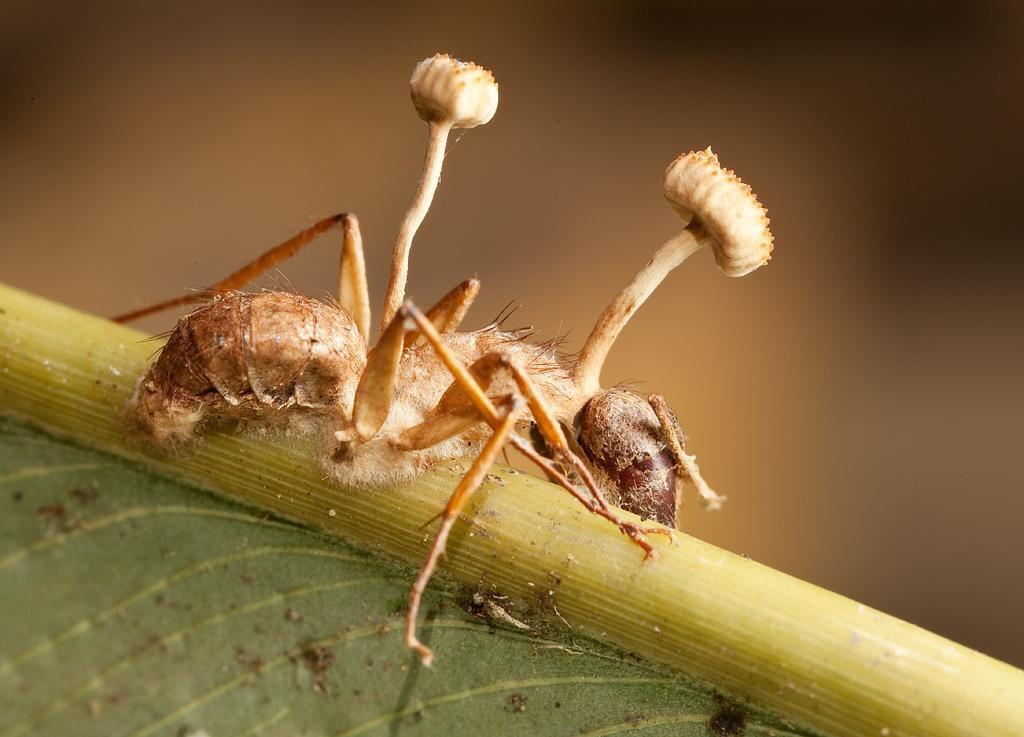
\includegraphics{ophiocordyceps.png}

}

\caption{Ophiocordyceps Unilaterialis}

\end{figure}%

\section{Question 2}\label{question-2}

To attempt to find a homologous protein, I inputted the accession number
into NCBI's tblastn search, using the est database, and did not add any
limits or restrictions.

My BLAST results were as followed:

\begin{figure}[H]

{\centering 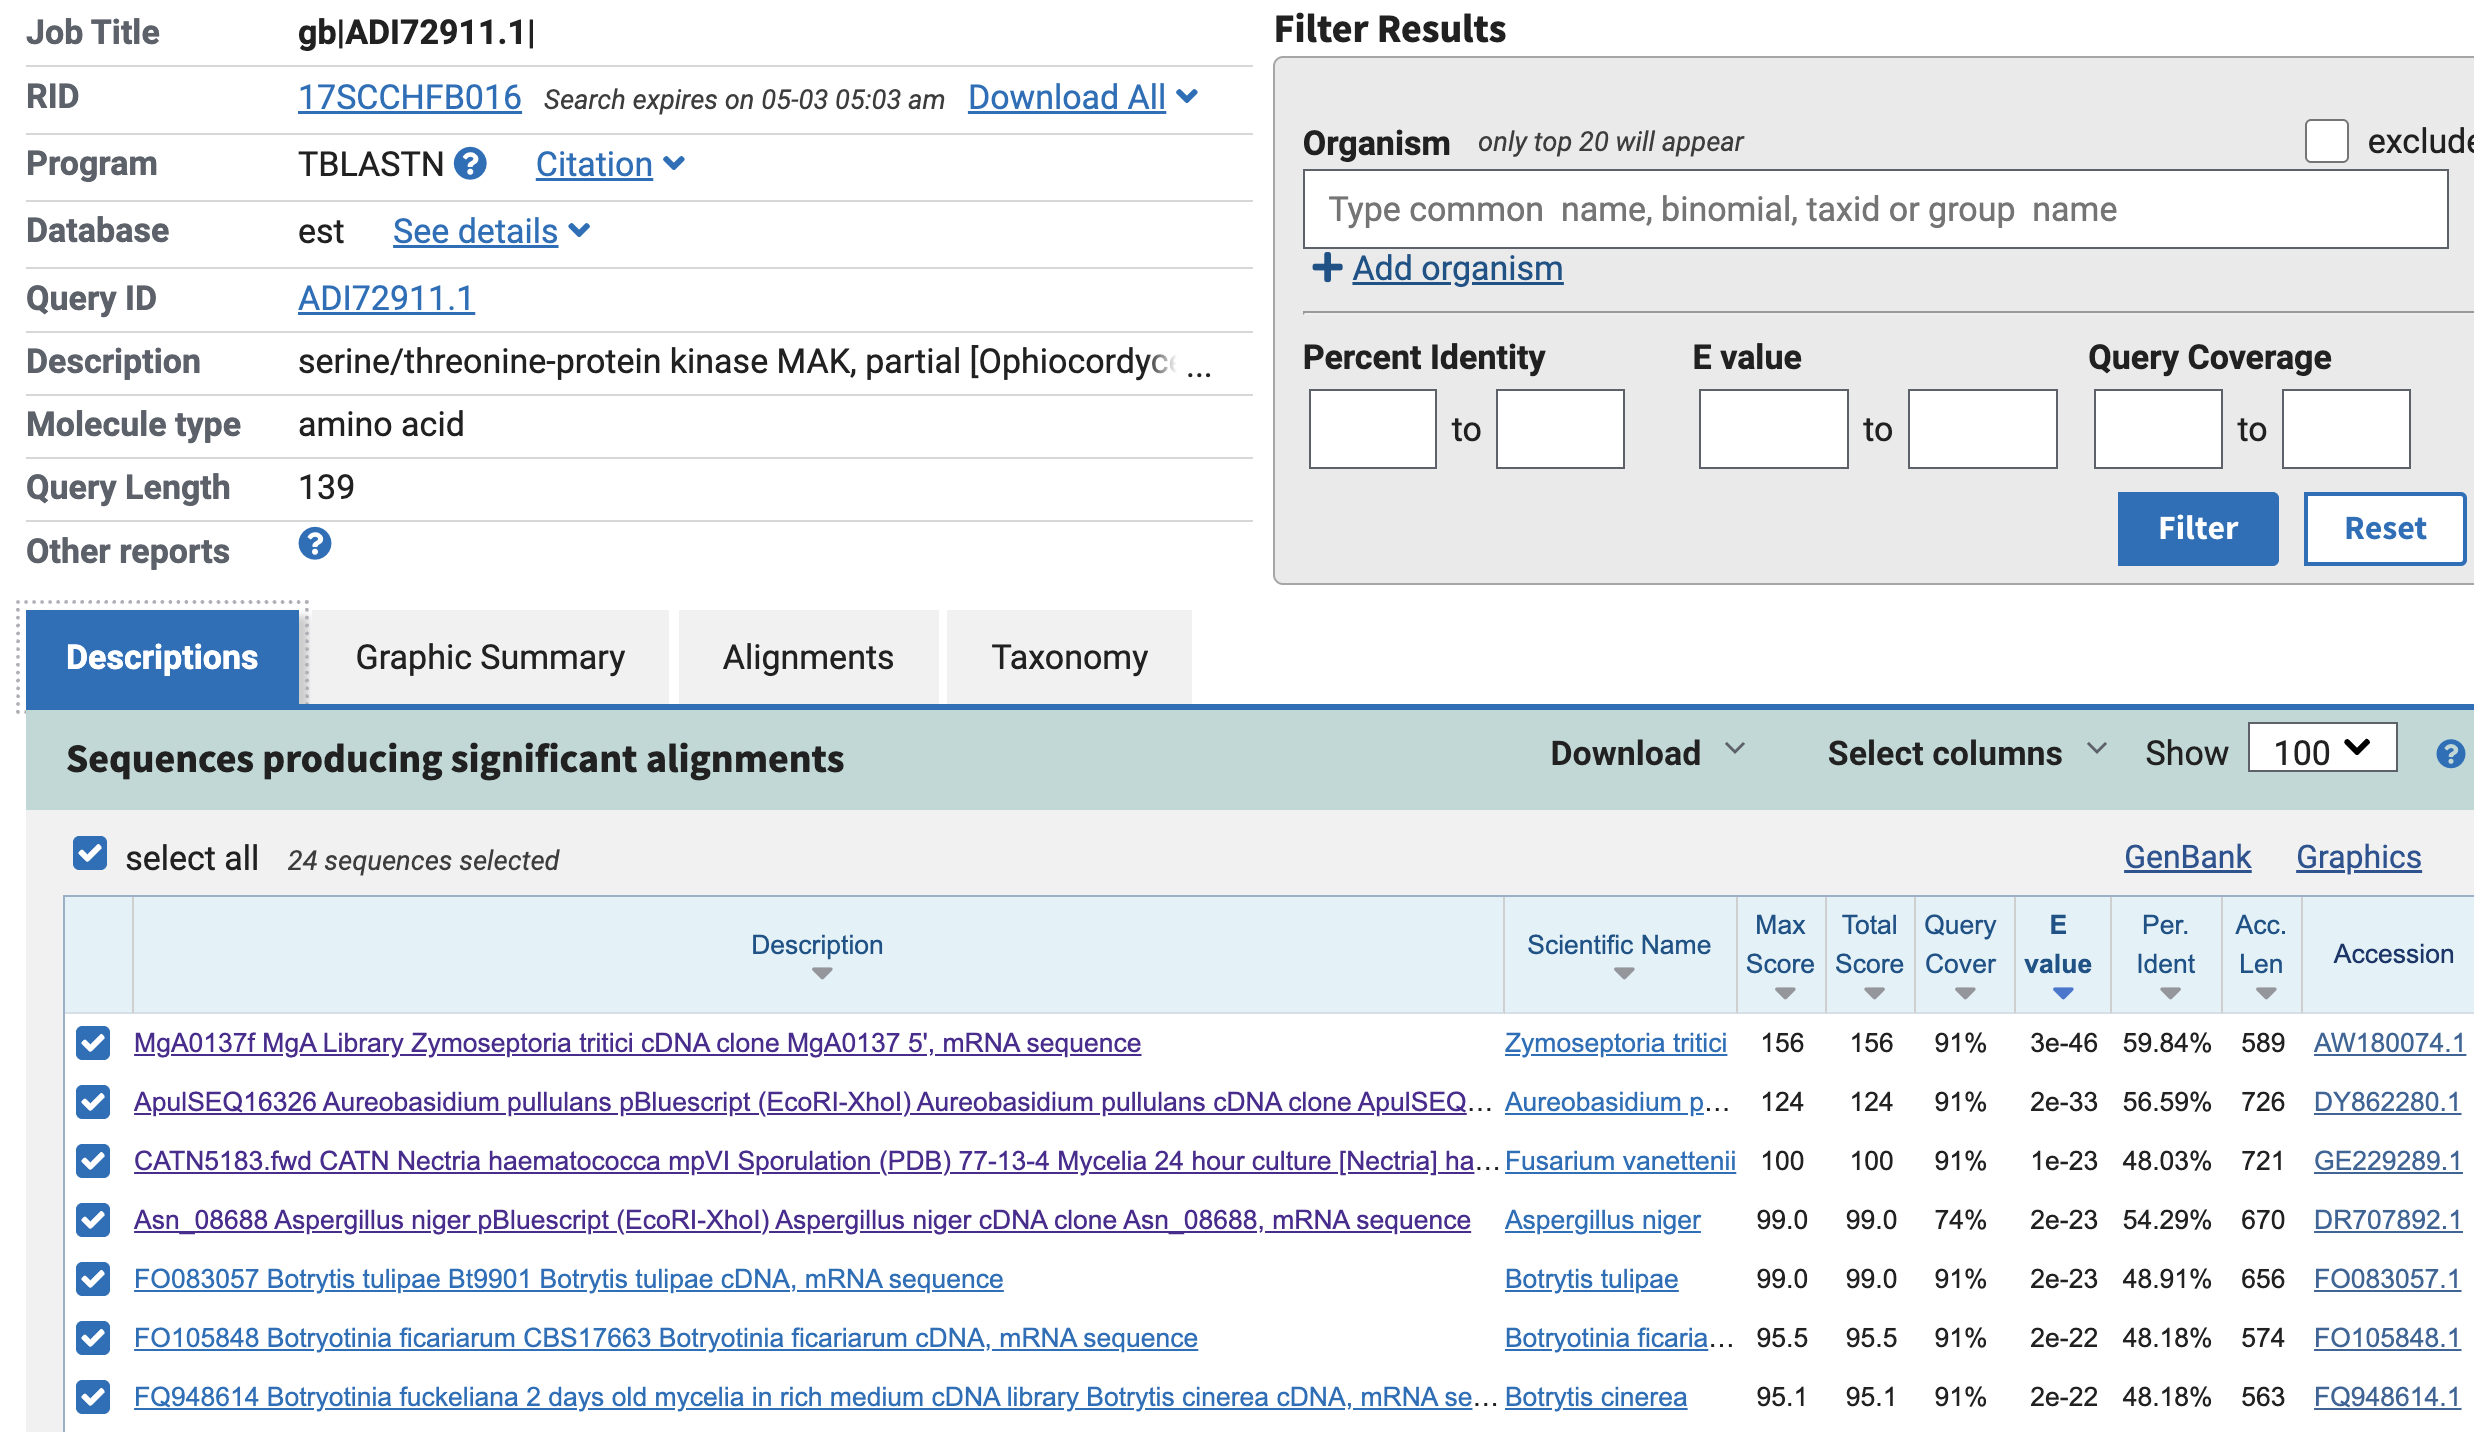
\includegraphics{original protein blast results.png}

}

\caption{BLAST results, original query}

\end{figure}%

I decided to focus on the first result, ``MgA0137f MgA Library
Zymoseptoria tritici cDNA clone MgA0137 5', mRNA sequence''.

\section{Question 3}\label{question-3}

Here is some information about the homolog I am looking into:

\textbf{FASTA format sequence, translated using EMBOSS Transeq}:
AW180074.1\_1 MgA0137f MgA Library Zymoseptoria tritici cDNA clone
MgA0137 5', mRNA sequence
RQLSVNSQGNHYAEIHRQEAERALVGASALKSPTGSQRESFFSHLRKRARRLSGRNSGVI
TPSMDAMETSAGCVPWAANKQTTFDTHSIASAAADPSSDPNFAELDRALQSVRYSLDAAA
NATQQARKPTNRVVEQPSLKRHHSLPHGVRHKTNPTTVYHDEH*STPRAADTRPPTKKKN
SRRSHELSASRRTAFSX

DNYQSTHRAITTPKFTGRKLSVLWLAQALSSHRLAAKEKASSLICARGREDFPAATQVSS
HLQWMLWKPALGAFLGLLTNKPPSTPTRSRLPQPIRHQTPISLSWIVHCKVYDTAWMPPR
TRLNKLGSLRTA\emph{LSNHH}SVTTRFLTALDTRPTQPPYTTTSTEARHEQPIQDPRRRRRI
LDEVMNSAHLAARRSR

TIISQLTGQSLRRNSPAGS\emph{ACSGWRKRSQVTDWQPKRKLLLSSAQEGEKTFRPQLRCHH
TFNGCYGNQRWVRSLGC}QTNHLRHPLDRVCRSRSVIRPQFR\emph{AGSCTAKCTIQPGCRRE
RDSTS}EAYEPRS\emph{ATIIEASPLASSRR}TQDQPNHRIPRRALKHATSSRYKTPDEEEEF
STKS*TQRISPHGVLX

RERRAARCAEFMTSSRILLLRRGSCIGCSWRASVLVVVYGGWVGLVSNAVRKRVVTLQ*W
LLNYAVRRLPSLLSRVRGGIQAVSYTLQCTIQLSEIGV\textbf{RIGCGRRDRVGVEGGLFVSS
PRNAPSAGFHSIH\emph{RCDDT}VAAGKSSRPLAQMREEAFSLAASR\emph{LESACANQSTLSFLP
VNFGVVIAL}VD}LS

SRTPCGEMR\emph{VHDFVENSSSSSGVLYRLLVACFSARRGIRWLGWSCV}RREEASGDASMM
VAQLRGS\emph{AS}LVESRSRRHPGCIVHFAVHDPAQRNWGLMTDRLRQTRSSGCRRWFVC\emph{Q
PKERTQRWFP}HPLKV**HLSCGRKVFSPSCADERRSFLFGCQSVT\emph{ERLRQPEHAQLPA
GEFRRSDCPVS}LIIVX

ENAVRRDALSS\emph{LRREFFFFVGGLVSAARGVLQCSSWYTVVGLVLCLTP}GSEW\emph{RFNDG
CSTTRFVGFLAC}VAFAAASRLYRTLCSARSSSAKLGSDDGSAAADAIEWVSKVVCLLAA
QGTHPALVSIASIEGVMTPELRPESLLALLRR\emph{EKKLSLWLPVGDLRALAPTRARSASCR
}ISA**LPCELTDNCR

\textbf{Name}: MgA0137f MgA Library Zymoseptoria tritici cDNA clone
MgA0137 5', mRNA sequence

\textbf{Species Derived from}: Zymoseptoria tritici : this is a
pathogenic fungus that attacks wheat plants. It is resistant to multiple
fungicides, and causes septoria leaf blotch.

\begin{figure}[H]

{\centering 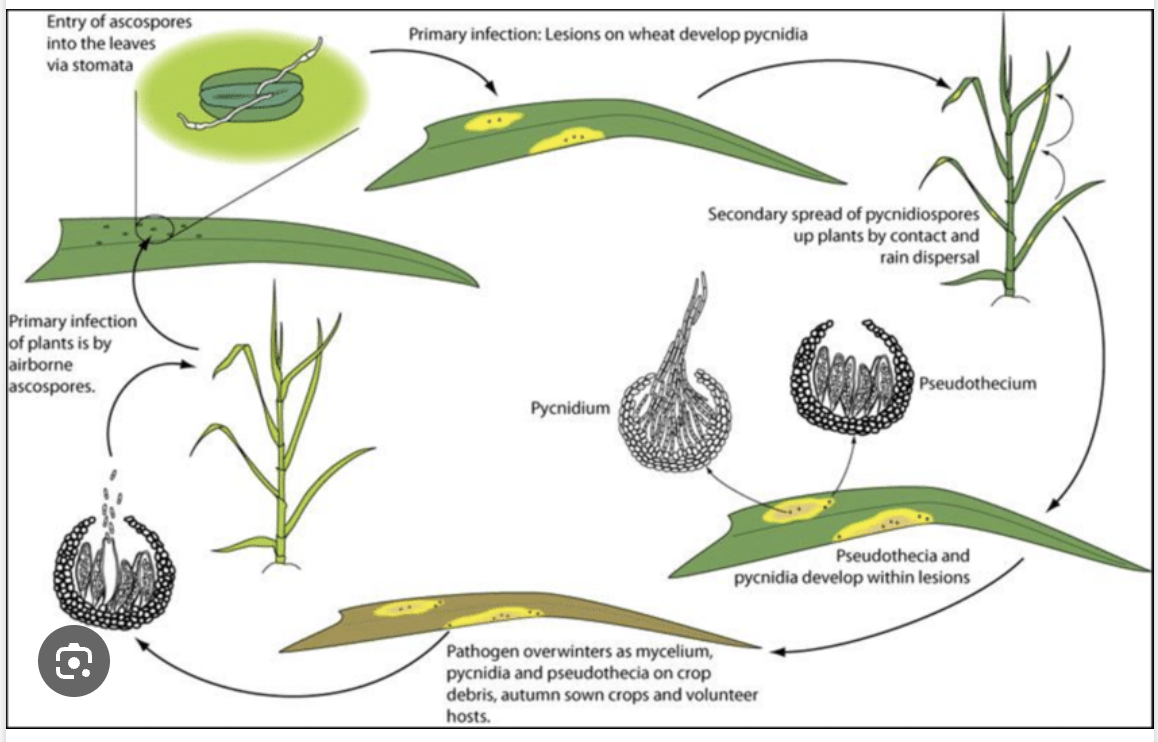
\includegraphics{zymoseptoria tritici.png}

}

\caption{Zymoseptoria Triciti}

\end{figure}%

\section{Question 4}\label{question-4}

To determine if my protein is novel, I used the ``blastp'' tool and
NCBI's nr database and ran the above FASTA format sequence through it.

My results were as followed:

\begin{figure}[H]

{\centering 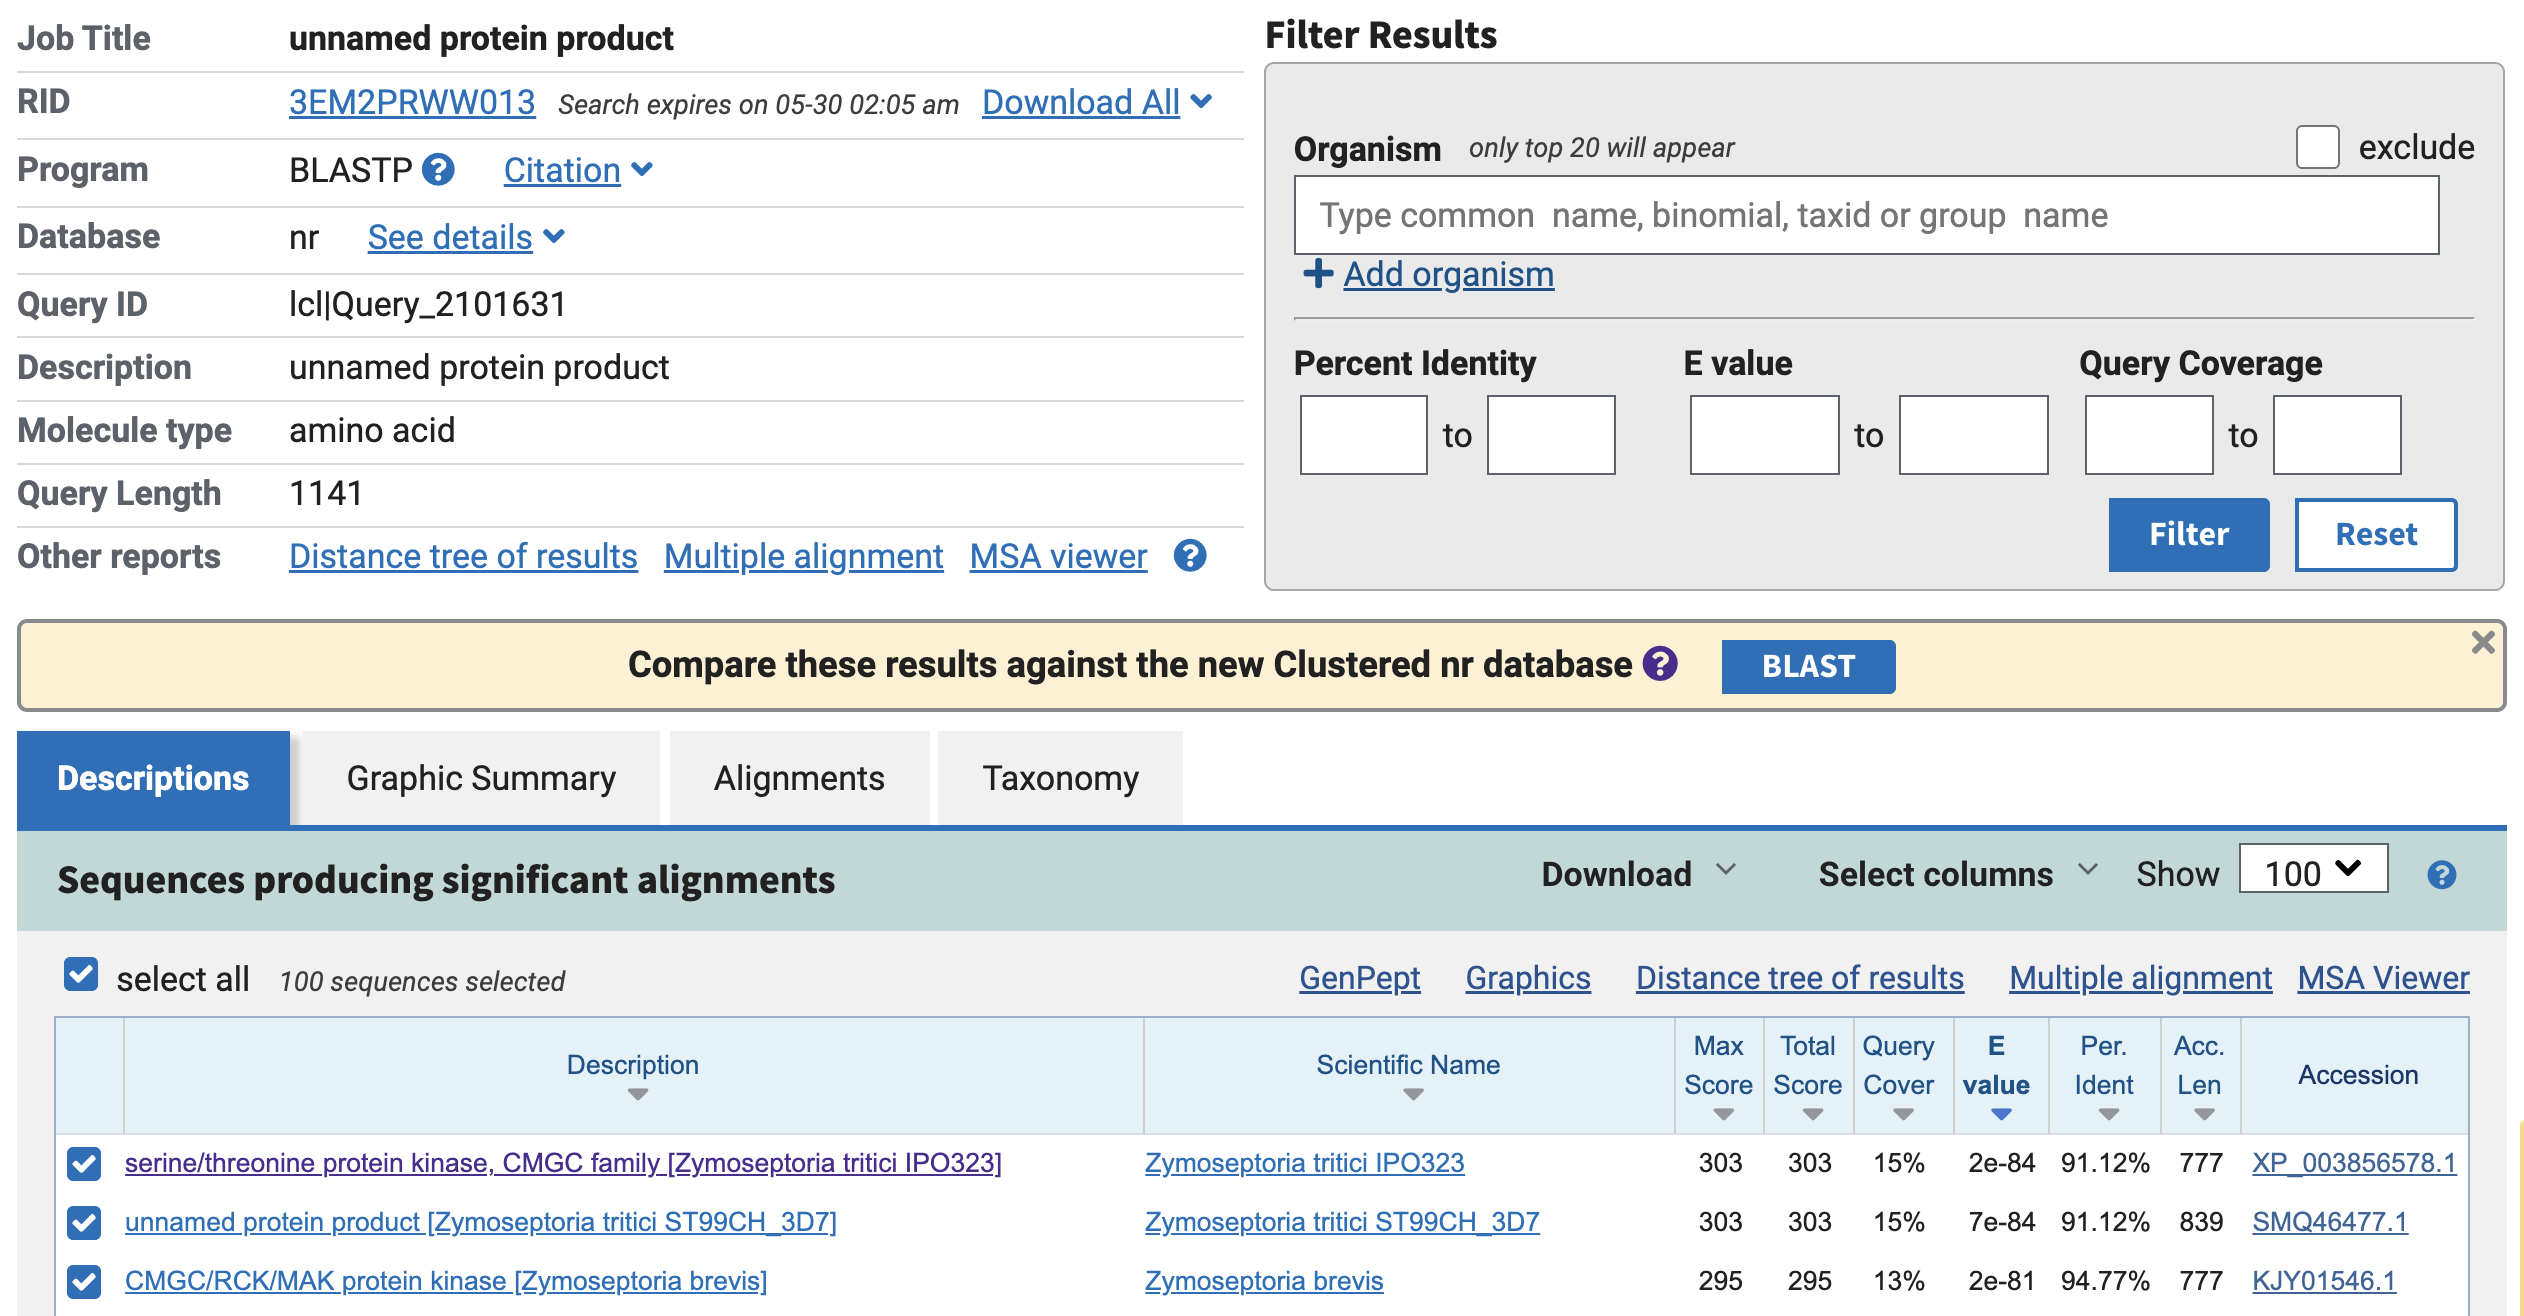
\includegraphics{novel protein blast results.png}

}

\caption{BLAST results, novel query}

\end{figure}%

There is no match with 100\% identity!

\section{Question 5}\label{question-5}

I will use MUSCLE at EBI to produce a multiple sequence alignment of the
following proteins:

\emph{My novel protein}

\texttt{\textgreater{}}Zymoseptoria unknown protein (novel protein from
BLAST results)
RQLSVNSQGNHYAEIHRQEAERALVGASALKSPTGSQRESFFSHLRKRARRLSGRNSGVITPSMDAMETSAGCVPWAANKQTTFDTHSIASAAADPSSDPNFAELDRALQSVRYSLDAAANATQQARKPTNRVVEQPSLKRHHSLPHGVRHKTNPTTVYHDEHSTPRAADTRPPTKKKNSRRSHELSASRRTAFSXDNYQSTHRAITTPKFTGRKLSVLWLAQALSSHRLAAKEKASSLICARGREDFPAATQVSSHLQWMLWKPALGAFLGLLTNKPPSTPTRSRLPQPIRHQTPISLSWIVHCKVYDTAWMPPRTRLNKLGSLRTALSNHHSVTTRFLTALDTRPTQPPYTTTSTEARHEQPIQDPRRRRRILDEVMNSAHLAARRSRTIISQLTGQSLRRNSPAGSACSGWRKRSQVTDWQPKRKLLLSSAQEGEKTFRPQLRCHHTFNGCYGNQRWVRSLGCQTNHLRHPLDRVCRSRSVIRPQFRAGSCTAKCTIQPGCRRERDSTSEAYEPRSATIIEASPLASSRRTQDQPNHRIPRRALKHATSSRYKTPDEEEEFSTKSTQRISPHGVLXRERRAARCAEFMTSSRILLLRRGSCIGCSWRASVLVVVYGGWVGLVSNAVRKRVVTLQWLLNYAVRRLPSLLSRVRGGIQAVSYTLQCTIQLSEIGVRIGCGRRDRVGVEGGLFVSSPRNAPSAGFHSIHRCDDTVAAGKSSRPLAQMREEAFSLAASRLESACANQSTLSFLPVNFGVVIALVDLSSRTPCGEMRVHDFVENSSSSSGVLYRLLVACFSARRGIRWLGWSCVRREEASGDASMMVAQLRGSASLVESRSRRHPGCIVHFAVHDPAQRNWGLMTDRLRQTRSSGCRRWFVCQPKERTQRWFPHPLKVHLSCGRKVFSPSCADERRSFLFGCQSVTERLRQPEHAQLPAGEFRRSDCPVSLIIVXENAVRRDALSSLRREFFFFVGGLVSAARGVLQCSSWYTVVGLVLCLTPGSEWRFNDGCSTTRFVGFLACVAFAAASRLYRTLCSARSSSAKLGSDDGSAAADAIEWVSKVVCLLAAQGTHPALVSIASIEGVMTPELRPESLLALLRREKKLSLWLPVGDLRALAPTRARSASCRISALPCELTDNCR

\emph{My original sequence for ophiocordyceps:}

\texttt{\textgreater{}}ADI72911.1 serine/threonine-protein kinase MAK,
partial {[}Ophiocordyceps unilateralis{]}
WQEAERALSGANGRKSPTGTLLESFFSHLRKRARRLSGRNQGPMSPGAEDLEANAGCAPWSSNRGSIQEPQPIEAVASDPSSDPNFAELDRALQNVRYSLDATANTSNNQPKHPTKMASNPSLKRHQSSHSGPAPSRKP

\textbf{Other proteins of interest, based on BLAST results of original
and novel proteins:}

\emph{1.} \texttt{\textgreater{}}KAK4508075.1 hypothetical protein
PRZ48\_001812 {[}Zasmidium cellare{]}
MTVAYDMSYRGWSSSSQSAACLEDKFEIIKDIGDGSFGSVSLGRTRSAGAHIVRRGTMVAIKTMKKTFENFAQCMELREIIFLKSLPNHPHLVPAYDIFLDPLSRKLHIAMEYMDGNLYQLMKARDHKPLDGTSVKSILFQILGGLEHIHDHHFFHRDIKPENILVSTSAPDTGNTFKRYSQLVTPPSTPPAYSIKIADFGLARETQSRVPYTTYVSTRWYRAPEVLLRAGEYSAPVDIWAVGAMAVEIATLKPLFPGGNEVDQVWRVCEIMGSPGSWVNKHGQKVGGGEWKDGIKLAQKLGFSFPKMAPHSLETVLPAPQWPASLAQFVTWCLMWDPKVRPTSRQALEHEYFRDAIDPLRPKSSGRALGRKGSTLGNNDPVDAQTLSTKTSLWFRKSLGARDTGAAPAVPEHMQLAQTQSPRPSPVHAQTTDPAAYVSKNRPAATKRATWTNGAASNAAPIPILPSIRPISPLPDQSVAQANARRTEQPEERPGKKIGRQLSVNSQGNHYADIHRQEAERALTGANGLKSPTGSQRESFFSHLRKRARRLSGRNQGPMSPGAEDIEASVGCAPWSTNNRGSIQEPQPIAPAAADPSTDPNFAELDRALQNVRYSLDAAANPANMQPKHPTKMPSNQSLKRHHSLPYGKEEIMSQTGGSTSNRTRRSLRHAPSSRYETPCEEDELLDEALASVHAAATRLDKGTSNVAGTYQPSRPPIGHVTSEPVYPAPYLTPSHSKDQMNVTYTSNEYTPSKAIDIPPMRPQQKAVVNPQWPTPPYDENDWASAAAASIFATQAQFR

\emph{2.} \texttt{\textgreater{}}XP\_047755397.1 Sporulation protein
kinase pit1 {[}Fulvia fulva{]}
MTVAYDNMSYRGWSSQSHSAVCLEDKFEILKDIGDGSFGSVTLGRTRGAGAHLVRRGTLVAIKTMKKTFENFAQCMELREVIFLKSLPNHPHLVPAYDIFLDPLSKKLHIAMEYMDGNLYQLMKARDHKPLDGTSVKSILFQILEGLEHIHDHHFFHRDIKPENILVSTSAPEAGNTFKRYSQLVTPPSTPPTYSIKIADFGLARETHSRVPYTTYVSTRWYRAPEVLLRAGEYSAPVDIWAIGAMAVEIATLKPLFPGGNEVDQVWRVCEIMGSPGSWVSKHGQKVGGGEWKEGIKLAQKLGFSFPKMAPHSMETVLPAPQWPASLAHFITWCLLWDPKNRPTSRQALEHEYFRDAVDPLRPKSSAAHALGRKQSTLVNNDSSEGLPMLSTKTSSWFRKSMGARENVAPAVPEHVQAYQNSSPRPSPVHANTTDPALVAAKGRPAATKRATWTNGAANNAAPIPILPSIRPISPLPDATVAQASTRRAEQSDERPGKKIGRQLSVNSQGNHYADMHRQEAERALTGATGLQSPTGSQRESFFSHLRKRARRLSGRNSGPMSPSAEDAEANVGCAPWASNNRQSVQEPQSIASVAVDPSSDPNFAELDRALQNVRYSLDAAAGAANPQPKQPTKMASNPTLKRHHSVPCSKEEVTSNPSMANRTRRSLRHAPSSRYETPCEEDELLDEALSNAHQAAQNLDNAPSMNTTATYQPARPLLPQAISEPAYAAPYLTPSPSKDQMNISYGAMDYSPTKPVDIPSMRAQPKGVVDPQWPTPPYDENDWASAAAASIFATQRAYQQ

\emph{3.} \texttt{\textgreater{}}KJY01546.1 CMGC/RCK/MAK protein kinase
{[}Zymoseptoria brevis{]}
MTVAYENMSYRGWSSGSHSAAVCLEDKFEIIKDIGDGSFGSVTLGRTRSAGAHLVRRNTLVAIKTMKKTFENFAQCMELREVIFLKTLPSHPHLVPAYDIFLDPLSKKLHIAMEHMDGNLYQLMKARDHKPLDESSVKSILFQILEGLEHIHDHSFFHRDIKPENILVSTSAHDTGSAFKRYSSLVTPPSTPPAYTIKIADFGLARETHSRVPYTTYVSTRWYRAPEVLLRAGEYSAPVDIWAIGAMAVEIATLKPLFPGGNEVDQVWRVCEVMGSPGAWVNKHGQKVGGGEWKEGIKLAQKLGFSFPKMAPHSLETVLPSPQWPASLANFITWCLMWDPKVRPTSRQALEHEYFQNALDPLAPKSSSRAQSRASVRHDSDLPTKTASWFRKSLGPRDAAPPAVPQHNSEPLATQPMPDPMESSPAPKVKPMAAKRATWAHGNANAAPMPILPSIRPISPLPDAITAHANARHIDQPPQEVSPSKKIGRQLSVNSQGNHYAEIHRQEAERALVGASALKSPTGSQRESFFSHLRKRARRLSGRNSGVITPSMDAMETNAGCVPWAANKQPVFDTHSVASAAADPSSDPNFAELDRALQSVRYSLDAAANATQQARKPTNRVVSNPSLKRHHSLPHGVDDKTQANHRIPRRALKHATSSRYETPDEEEELLDEVMTSAHLAARRLDNEQLSRPPLPHVISEPVTVYTAPYLTPSHSKDQMSLDYVTQGPAPTNAVEIPPRRQPSNSKNNPQWPTPPYDENDWAAAAAASIFATQRAYQ

\emph{4.} \texttt{\textgreater{}}KAK4981489.1 hypothetical protein
LTR28\_003093, partial {[}Elasticomyces elasticus{]}
MRRSDAEEKASRKIGRQLSVASHGNHYADAHRHEAEQALNGRNGLASPTSSQRGSFFAHLRKRARRLSGRNQAPVSPSVDDIEASAGCAPWASNRQSMAIESLAITTHATDPSSDPNFAELDRALQNVRYSLDAGSYSNNNVQKPVQKVPSNPMLKRHHSLPFGQDERISPVPAVNGPISSRTRRSVRQAPHPGHRYETPDEEEELLDEVLASAHRAARRLDRYIQQDNSPLPSVTSQQERARPPVQQVTSDPGCFVPYLTPSPSKDRNG

\emph{5. } \texttt{\textgreater{}}KAI5369935.1 putative
serine/threonine-protein kinase, active {[}Septoria linicola{]}
MTVAYDMSYRGWSSGSQSAVCLEDKFEILKDIGDGSFGSVTLGRTRGAGAHIVRRGTLVAIKTMKKTFESFSQCMELREVIFLRTLPNHPHLVPAYDIFLDPLSKKLHIAMEYMDGNLYQLMKARDHKPLDCSSVKSILFQILGGLEHIHDHSFFHRDIKPENILVSTSAPDTGSAFKRYSALVTPPSTPPAYSIKIADFGLARETHSRVPYTTYVSTRWYRAPEVLLRAGEYSAPVDIWAVGAMAVEIATLKPLFPGGNEVDQVWRVCEIMGSPGSWVNKHGNIVGGGEWKDGIKLAQKLGFSFPKMAPHSLETVLCAPHWPASLAQLVTWCLMWDPKVRPTSRQALEHEFFNDALDPLRPKSAATKTLGRKASTHIGATDGSDGIPTLTTKTSSWFRKSLGPRDNSAPSVPEYAQVSHTSSPRPTPAPSVPLESTASSKQARPGATKRATWTNGASTAAPIPILPSIRPISPLPDASVAQASVRRTEQPDERPGKKIGRQLSVNSQGNHYAELHRQEAERALNGASGLKSPTGSQRESFFSHLRKRARRFSGKPSGLASPTAEDMEANVGCAPWTTNRQSIPDAQAIAPTAADPSVDPNFAELDRALQSVRYSLDATAGAMPTQPKPPVKMASNPALKRHHSLPYGKEELSVVNRTRRSVKQAPSNIRYETPCEEDELLDEAIASAHQAVTRLDNGITQPARPHLPHVTSEPTYNVPYLTPSPSKDHMAVDFVANDCTPSKPVNIPAIRAQDKAVVNPQWPTPPYDENDWASGVAASIFATQAAFR

\emph{Alignment} Here is the alignment I obtained after running the
above 7 proteins through MUSCLE at EBI (it's quite long):

CLUSTAL msa by MUSCLE:

Zymoseptoria\_unknown\_protein
RQLSVNSQGNHYAEIHRQEAERALVGASALKSPTGSQRESFFSHLRKRARRLSGRNSGVI
KAK4981489.1
------------------------------------------------------------ KJY01546.1
MTVAYENMSYRGWSSGSHSAAVCLEDKFEIIKDIGDGSFGSVTLGRTRSAGAHLVRRNTL ADI72911.1
------------------------------------------------------------
KAI5369935.1
MTVAYD-MSYRGWSSGSQSA-VCLEDKFEILKDIGDGSFGSVTLGRTRGAGAHIVRRGTL
KAK4508075.1
MTVAYD-MSYRGWSSSSQSA-ACLEDKFEIIKDIGDGSFGSVSLGRTRSAGAHIVRRGTM
XP\_047755397.1
MTVAYDNMSYRGWSSQSHSA-VCLEDKFEILKDIGDGSFGSVTLGRTRGAGAHLVRRGTL

Zymoseptoria\_unknown\_protein
TPSMDAMETSAGCVPWAANKQTTFDTHSIASAAADPSSDPNFAELDRALQSVRYSLDAAA
KAK4981489.1
------------------------------------------------------------ KJY01546.1
VAIKTMKKTFENFAQCMELREVIFLKTLPSHPHLVPAYDIFLDPLSKKLHIAMEHMDGNL ADI72911.1
------------------------------------------------------------
KAI5369935.1
VAIKTMKKTFESFSQCMELREVIFLRTLPNHPHLVPAYDIFLDPLSKKLHIAMEYMDGNL
KAK4508075.1
VAIKTMKKTFENFAQCMELREIIFLKSLPNHPHLVPAYDIFLDPLSRKLHIAMEYMDGNL
XP\_047755397.1
VAIKTMKKTFENFAQCMELREVIFLKSLPNHPHLVPAYDIFLDPLSKKLHIAMEYMDGNL

Zymoseptoria\_unknown\_protein
NATQQARKPTNRVVEQPSLKR-HHSLPHGVRHKTNPTTVYHDEHSTPRAADTRPPTKKKN
KAK4981489.1
------------------------------------------------------------ KJY01546.1
YQLMKARD--HKPLDESSVKSILFQILEGLEHIHDHSFFHRDIKPENILVSTSAHDTGSA ADI72911.1
------------------------------------------------------------
KAI5369935.1
YQLMKARD--HKPLDCSSVKSILFQILGGLEHIHDHSFFHRDIKPENILVSTSAPDTGSA
KAK4508075.1
YQLMKARD--HKPLDGTSVKSILFQILGGLEHIHDHHFFHRDIKPENILVSTSAPDTGNT
XP\_047755397.1
YQLMKARD--HKPLDGTSVKSILFQILEGLEHIHDHHFFHRDIKPENILVSTSAPEAGNT

Zymoseptoria\_unknown\_protein
SRRSHELSASRRTAFSXDNYQSTHRAITTPKFTGRKLSVLWLAQALSSHRLAAKEKASSL
KAK4981489.1
------------------------------------------------------------ KJY01546.1
FKRYSSLVTPPSTPPAYT------------------IKIADFGLARETHSRVPYTTYVST ADI72911.1
------------------------------------------------------------
KAI5369935.1
FKRYSALVTPPSTPPAYS------------------IKIADFGLARETHSRVPYTTYVST
KAK4508075.1
FKRYSQLVTPPSTPPAYS------------------IKIADFGLARETQSRVPYTTYVST
XP\_047755397.1
FKRYSQLVTPPSTPPTYS------------------IKIADFGLARETHSRVPYTTYVST

Zymoseptoria\_unknown\_protein
ICARGREDFPAATQVSSHLQWMLWKPALGAFLGLLTNKPPSTPTRSRLPQPIRHQTPISL
KAK4981489.1
------------------------------------------------------------ KJY01546.1
RWYRAPEVLLRAGEYSAPVD--IW--AIGAMAVEIATLKPLFPGGNEVDQVWR------- ADI72911.1
-----------------------W------------------------------------
KAI5369935.1
RWYRAPEVLLRAGEYSAPVD--IW--AVGAMAVEIATLKPLFPGGNEVDQVWR-------
KAK4508075.1
RWYRAPEVLLRAGEYSAPVD--IW--AVGAMAVEIATLKPLFPGGNEVDQVWR-------
XP\_047755397.1
RWYRAPEVLLRAGEYSAPVD--IW--AIGAMAVEIATLKPLFPGGNEVDQVWR-------

Zymoseptoria\_unknown\_protein
SWIVHCKVYDTAWMPPRTRLNKLGSLRTALSNHHSVTTRFLTALDTRPTQPPYTTTSTEA
KAK4981489.1
------------------------------------------------------------ KJY01546.1
--VCEVMGSPGAWVNKHGQKVGGGEWKEGIKLAQKLGFSF-------------------- ADI72911.1
------------------------------------------------------------
KAI5369935.1
--VCEIMGSPGSWVNKHGNIVGGGEWKDGIKLAQKLGFSF--------------------
KAK4508075.1
--VCEIMGSPGSWVNKHGQKVGGGEWKDGIKLAQKLGFSF--------------------
XP\_047755397.1
--VCEIMGSPGSWVSKHGQKVGGGEWKEGIKLAQKLGFSF--------------------

Zymoseptoria\_unknown\_protein
RHEQPIQDPRRRRRILDEVMNSAHLAARRSRTIISQLTGQSLRRNSPAGSACSGWRKRSQ
KAK4981489.1
------------------------------------------------------------ KJY01546.1
--------PKMAPHSLETVLPSPQWPASLANFITWCLMWDPKVRPTSRQALEHEYF-QNA ADI72911.1
------------------------------------------------------------
KAI5369935.1
--------PKMAPHSLETVLCAPHWPASLAQLVTWCLMWDPKVRPTSRQALEHEFF-NDA
KAK4508075.1
--------PKMAPHSLETVLPAPQWPASLAQFVTWCLMWDPKVRPTSRQALEHEYF-RDA
XP\_047755397.1
--------PKMAPHSMETVLPAPQWPASLAHFITWCLLWDPKNRPTSRQALEHEYF-RDA

Zymoseptoria\_unknown\_protein
VTDWQPKRKLLLSSAQEGEKTFRPQLRCHHTFNGCYGNQRWVR-SLGCQTNHLRHPLDRV
KAK4981489.1
------------------------------------------------------------ KJY01546.1
LDPLAPKSS-----SRAQSRASVRHD-----SDLPTKTASWFRKSLGPRDA-APPAVPQH ADI72911.1
------------------------------------------------------------
KAI5369935.1
LDPLRPKSAATKTLGRKASTHIGATDGSDGIPTLTTKTSSWFRKSLGPRDN-SAPSVPEY
KAK4508075.1
IDPLRPKSS-GRALGRKGS-TLGNNDPVDA-QTLSTKTSLWFRKSLGARDTGAAPAVPEH
XP\_047755397.1
VDPLRPKSSAAHALGRKQS-TLVNNDSSEGLPMLSTKTSSWFRKSMGAREN-VAPAVPEH

Zymoseptoria\_unknown\_protein
CRSRSVIRPQ-FRAGSCTAKCTIQPGCRRERDSTSEAYEPRSATIIEASPLASSRRTQDQ
KAK4981489.1
------------------------------------------------------------ KJY01546.1
NSEPLATQPMPDPMESSP------APKVKPMAAKRATWAHG-NANAAPMPILPSIR---- ADI72911.1
------------------------------------------------------------
KAI5369935.1
AQVSHTSSPRPTPAPSVPLESTASSKQARPGATKRATWTNG-ASTAAPIPILPSIR----
KAK4508075.1
MQLAQTQSPRPSPVHAQTTDPAAYVSKNRPAATKRATWTNGAASNAAPIPILPSIR----
XP\_047755397.1
VQAYQNSSPRPSPVHANTTDPALVAAKGRPAATKRATWTNGAANNAAPIPILPSIR----

Zymoseptoria\_unknown\_protein
PNHRIPRRALKHATSSRYKTPDEEEEFSTKSTQRISPHGVLXRERRAARCAEFMTSSRIL
KAK4981489.1
--------------MRRSDAEE---KASRKIGRQLS------------------------ KJY01546.1
PISPLPDAITAHANARHIDQPPQEVSPSKKIGRQLS------------------------ ADI72911.1
------------------------------------------------------------
KAI5369935.1
PISPLPDASVAQASVRRTEQPDE--RPGKKIGRQLS------------------------
KAK4508075.1
PISPLPDQSVAQANARRTEQPEE--RPGKKIGRQLS------------------------
XP\_047755397.1
PISPLPDATVAQASTRRAEQSDE--RPGKKIGRQLS------------------------

Zymoseptoria\_unknown\_protein
LLRRGSCIGCSWRASVLVVVYGGWVGLVSNAVRKRVVTLQWLLNYAVRRLPSLLSRVRGG
KAK4981489.1
-----------------VASHGNHYADAHRHEAEQALN---------------------- KJY01546.1
-----------------VNSQGNHYAEIHRQEAERALV---------------------- ADI72911.1
------------------------------QEAERALS----------------------
KAI5369935.1
-----------------VNSQGNHYAELHRQEAERALN----------------------
KAK4508075.1
-----------------VNSQGNHYADIHRQEAERALT----------------------
XP\_047755397.1
-----------------VNSQGNHYADMHRQEAERALT----------------------

Zymoseptoria\_unknown\_protein
IQAVSYTLQCTIQLSEIGVRIGCGRRDRVGVEGGLFVSSPRNAPSAGFHSIHRCDDTVAA
KAK4981489.1
-----------------------------GRNG---LASPTSSQRGSFFAHLRKRARRLS KJY01546.1
-----------------------------GASA---LKSPTGSQRESFFSHLRKRARRLS ADI72911.1
-----------------------------GANG---RKSPTGTLLESFFSHLRKRARRLS
KAI5369935.1
-----------------------------GASG---LKSPTGSQRESFFSHLRKRARRFS
KAK4508075.1
-----------------------------GANG---LKSPTGSQRESFFSHLRKRARRLS
XP\_047755397.1
-----------------------------GATG---LQSPTGSQRESFFSHLRKRARRLS

Zymoseptoria\_unknown\_protein
GKSSRPLAQMREEAFSLAASRLESACANQSTLSFLPVNFGVVIALVDLSSRTPCGEMRVH
KAK4981489.1
GRNQAPVSPSVDD---------------------IEASAG-------------CAP---- KJY01546.1
GRNSGVITPSMDA---------------------METNAG-------------CVP---- ADI72911.1
GRNQGPMSPGAED---------------------LEANAG-------------CAP----
KAI5369935.1
GKPSGLASPTAED---------------------MEANVG-------------CAP----
KAK4508075.1
GRNQGPMSPGAED---------------------IEASVG-------------CAP----
XP\_047755397.1
GRNSGPMSPSAED---------------------AEANVG-------------CAP----

Zymoseptoria\_unknown\_protein
DFVENSSSSSGVLYRLLVACFSARRGIRWLGWSCVRREEASGDASMMVAQLRGSASLVES
KAK4981489.1
-------------------------------WAS-NRQSMAIE----------------- KJY01546.1
-------------------------------WAA-NKQPVF-D----------------- ADI72911.1
-------------------------------WSS-NRGSIQ-E-----------------
KAI5369935.1
-------------------------------WTT-NRQSIP-D-----------------
KAK4508075.1
-------------------------------WSTNNRGSIQ-E-----------------
XP\_047755397.1
-------------------------------WASNNRQSVQ-E-----------------

Zymoseptoria\_unknown\_protein
RSRRHPGCIVHFAVHDPAQRNWGLMTDRLRQTRSSGCRRWFVCQPKERTQRWFPHPLKVH
KAK4981489.1
-----SLAITTHATDPSSDPNFAELDRALQNVRYSLDAGSYSNNNVQK------PVQKV- KJY01546.1
-----THSVASAAADPSSDPNFAELDRALQSVRYSLDAAANATQQARK------PTNRV- ADI72911.1
-----PQPIEAVASDPSSDPNFAELDRALQNVRYSLDATANTSNNQPK------HPTKM-
KAI5369935.1
-----AQAIAPTAADPSVDPNFAELDRALQSVRYSLDATAGAMPTQPK------PPVKM-
KAK4508075.1
-----PQPIAPAAADPSTDPNFAELDRALQNVRYSLDAAANPANMQPK------HPTKM-
XP\_047755397.1
-----PQSIASVAVDPSSDPNFAELDRALQNVRYSLDAAAGAANPQPK------QPTKM-

Zymoseptoria\_unknown\_protein
LSCGRKVFSPSCADERRSFLFGCQSVTERLRQPEHAQLPAGEFRRSDCPVSLIIVXENAV
KAK4981489.1
---------PSNPMLKR-----------------HHSLPFGQDERISPVPAVNGPISSRT KJY01546.1
---------VSNPSLKR-----------------HHSLPHGVDDKTQ-------ANHRIP ADI72911.1
---------ASNPSLKR-----------------HQSSHSG-------------------
KAI5369935.1
---------ASNPALKR-----------------HHSLPYGKEEL---------SVVNRT
KAK4508075.1
---------PSNQSLKR-----------------HHSLPYGKEEIMSQT---GGSTSNRT
XP\_047755397.1
---------ASNPTLKR-----------------HHSVPCSKEEVTSNP-----SMANRT

Zymoseptoria\_unknown\_protein
RRDALSSLRREFFFFVGGLVSAARGVLQCSSWYTVVGLVLCLTPGSEWRFNDGCSTTRFV
KAK4981489.1
RRS------------------------------------VRQAPHPGHRYETPDEEEELL KJY01546.1
RRA------------------------------------LKHATSS--RYETPDEEEELL ADI72911.1
------------------------------------------------------------
KAI5369935.1
RRS------------------------------------VKQAPSN-IRYETPCEEDELL
KAK4508075.1
RRS------------------------------------LRHAPSS--RYETPCEEDELL
XP\_047755397.1
RRS------------------------------------LRHAPSS--RYETPCEEDELL

Zymoseptoria\_unknown\_protein
GFLACVAFAAASRLYRTLCSARSSSAKLGSDDGSAAADAIEWVSKV--VCLLAAQGTHPA
KAK4981489.1
DEVLASAHRAARRLDRYIQQDNSPLPSVTSQQERARPPVQQVTSDP--GCFVPYLTPSPS KJY01546.1
DEVMTSAHLAARRL---------------DNEQLSRPPLPHVISEPVTVYTAPYLTPSHS ADI72911.1
--------------------------------------------------------PAPS
KAI5369935.1
DEAIASAHQAVTRL-------------DNGITQPARPHLPHVTSEP--TYNVPYLTPSPS
KAK4508075.1
DEALASVHAAATRL------DKGTS-NVAGTYQPSRPPIGHVTSEP--VYPAPYLTPSHS
XP\_047755397.1
DEALSNAHQAAQNL------DNAPSMNTTATYQPARPLLPQAISEP--AYAAPYLTPSPS

Zymoseptoria\_unknown\_protein
LVSIASIEGVMTPELRPESLLALLRREKKLSLWLPVGDLRALAPTRARSASCRISALPCE
KAK4981489.1
KDRNG------------------------------------------------------- KJY01546.1
KDQMSLDYVTQGPAPTNAVEIPPRRQPSNSKNNPQWPTPPYDENDWAAAAAASIFATQRA ADI72911.1
RKP---------------------------------------------------------
KAI5369935.1
KDHMAVDFVANDCTPSKPVNIPAIRAQDKAVVNPQWPTPPYDENDWASGVAASIFATQAA
KAK4508075.1
KDQMNVTYTSNEYTPSKAIDIPPMRPQQKAVVNPQWPTPPYDENDWASAAAASIFATQAQ
XP\_047755397.1
KDQMNISYGAMDYSPTKPVDIPSMRAQPKGVVDPQWPTPPYDENDWASAAAASIFATQRA

Zymoseptoria\_unknown\_protein LTDNCR KAK4981489.1 ------ KJY01546.1
YQ---- ADI72911.1 ------ KAI5369935.1 FR---- KAK4508075.1 FR----
XP\_047755397.1 YQQ---

\section{Question 6}\label{question-6}

Phylogenetic tree

\section{Question 7}\label{question-7}

Heatmap

\section{Question 8}\label{question-8}

\section{Question 9}\label{question-9}

Because the sequence of my novel protein is quite long, some shortening
is required before a multiple sequence alignment can be produced. It
needs to be less than or equal to 1000 AAs long for MUSCL at EBI to
process it.

I was unsure of the best way to shorten my sequence, so I asked ChatGPT
to do it for me. It identified a central 1000-amino acid segment that
avoids the N-terminal signal peptide and C-terminal polybasic tail,
which are less structured and may not be essential for the core
function.

The resulting novel sequence (zymoseptoria) I will run through ColabFold
is:

``VITPSMDAMETSAGCVPWAANKQTTFDTHSIASAAADPSSDPNFAELDRALQSVRYSLDAAANATQQARKPTNRVVEQPSLKRHHSLPHGVRHKTNPTTVYHDEH\emph{STPRAADTRPPTKKKNSRRSHELSASRRTAFSXDNYQSTHRAITTPKFTGRKLSVLWLAQALSSHRLAAKEKASSLICARGREDFPAATQVSSHLQWMLWKPALGAFLGLLTNKPPSTPTRSRLPQPIRHQTPISLSWIVHCKVYDTAWMPPRTRLNKLGSLRTALSNHHSVTTRFLTALDTRPTQPPYTTTSTEARHEQPIQDPRRRRRILDEVMNSAHLAARRSRTIISQLTGQSLRRNSPAGSACSGWRKRSQVTDWQPKRKLLLSSAQEGEKTFRPQLRCHHTFNGCYGNQRWVRSLGCQTNHLRHPLDRVCRSRSVIRPQFRAGSCTAKCTIQPGCRRERDSTSEAYEPRSATIIEASPLASSRRTQDQPNHRIPRRALKHATSSRYKTPDEEEEFSTKSTQRISPHGVLXRERRAARCAEFMTSSRILLLRRGSCIGCSWRASVLVVVYGGWVGLVSNAVRKRVVTLQWLLNYAVRRLPSLLSRVRGGIQAVSYTLQCTIQLSEIGVRIGCGRRDRVGVEGGLFVSSPRNAPSAGFHSIHRCDDTVAAGKSSRPLAQMREEAFSLAASRLESACANQSTLSFLPVNFGVVIALVDLSSRTPCGEMRVHDFVENSSSSSGVLYRLLVACFSARRGIRWLGWSCVRREEASGDASMMVAQLRGSASLVESRSRRHPGCIVHFAVHDPAQRNWGLMTDRLRQTRSSGCRRWFVCQPKERTQRWFP}HPLKVHLSCGRKVFSPSCADERRSFLFGCQSVTERLRQPEHAQLPAGEFRRSDCPVSLIIVXENAVRRDALSSLRREFFFFVGGLVSAARGVLQCSSWYTVVGLVLCLTPGSEWRFNDGCSTTRFVGFLACVAFAAASRLYRTLCSARSSSAKLGSDDGSAAADAIEWVSKVVCLLAAQGTHPALVSIASIEGVMTPELRPESLLALLRREKKLSLWLPVGDLRALAPTRARSASCRISALPCELTDN''

\section{Question 10}\label{question-10}




\end{document}
